
\section{The basics}

People who lend money often insist on being paid a rental rate. The rate depends on the period of the loan, the person, the currency, and a number of other factors. Loans are often resold into secondary markets and traded like any other financial asset. The study of money loans is called \textbf{fixed income} (or \textbf{fixed interest}) because the amount of money repaid is generally fixed by agreement, in comparison to other assets where future financial flows are uncertain.

Fixed income is useful to know:  The pricing and analysis of many other products incorporates information about the rental price of money, so it's difficult to understand what's going on with options or futures or more exotic things without knowing a bit about the debt markets.

Three objects will concern us here: \textbf{bonds}, \textbf{zero rates}, \textbf{forward rates}, and \textbf{swap rates}. Understanding these and how to convert between them is fundamental to understanding fixed income markets. We'll start by assuming that all loans are the same except for when they are taken out and repaid.

\subsection{Notation}
Start with some notation. Let $y(t)$ be the interest rate for a loan made now and repaid in $t$ years. The curve for all $t$ is called the \textbf{zero curve} and the component rates \textbf{zero rates}. This is short for `zero coupon', but don't worry about that for now.

Now let $f(t_1,t_2)$ be the interest rate for a loan made at time $t_1$ and paid back at time $t_2$. These are called \textbf{forward rates}.

Unless otherwise noted all rates from here will be continuously compounded. The appendix contains a reminder of how continuous compounding works and how to convert between discrete and continuous compounded rates so $N$ dollars borrowed at rate $y$ for $T$ periods will compound to

\[N\exp (yT) \]


\section{Converting between zero rates and forward rates}


\subsection{General case}

If we have two \textit{zero rates} $y(t_1)$ and $y(t_2)$ we can determine the forward rate $f(t_1,t_2)$ -- the interest rate on a loan taken out at $t_1$ and repaid at $t_2$ -- using an arbitrage argument. The essence of this argument is that it should cost the same to borrow from now to $t_1$, and then at the forward rate from $t_1$ to $t_2$, as it does to simply borrow from now to $t_2$. If this were not true there would be an arbitrage.

In more concrete terms it should cost the same to take out a loan for two years as to take out a loan for one year, and another in a years time at the forward rate (see figure \ref{frArb}) . This gives us the formula for forward rates:

\begin{figure}[htbp]
\begin{center}
  \includegraphics[width=5in]{pics/zt1t2_llb.png} \\
  \caption{Forward rate arbitrage: borrow long, lend short}
\label{frArb}
\end{center}
\end{figure}


\begin{center}
(loan for $t_2$ periods)  = (loan for $t_1$ periods)(loan for $t_2-t_1$ periods)
\[\Rightarrow \exp(y(t_2)t_2) = \exp(y(t_1)t_1)\exp(f(t_1,t_2)(t_2-t_1)) \]
We can solve to get any forward rate:
\begin{equation}f(t_1,t_2) = \frac{y(t_2)t_2-y(t_1)t_1}{t_2-t_1}  \label{fRates}\end{equation}
\end{center}


\subsection{Example} Suppose that $y(1) = 0.05$ and $y(2) = 0.075$. We can see immediately that

\[f(1,2) = \frac{0.075*2-0.05*1}{2-1} = 0.1 \]


Which is to say that the one year rate one year from now (from year one to year two) should be 10\%.

\subsection{Forward rate arbitrage}

If the forward and zero rates does not conform to \ref{fRates} there will be arbitrage. We'll work through a couple of examples to see how this works.

But what if it isn't? What if instead $f(1,2)=0.11$? Then we would have the following arbitrage:
\begin{center}
\begin{tabular}{|c|c|}
  \hline
  % after \\: \hline or \cline{col1-col2} \cline{col3-col4} ...
  time & transaction \\
  \hline
  now & Borrow \$1 for 2 years at 0.075 \\
   & Lend \$1 for 1 year at 0.05 \\
   \hline
  1 & Receive \$ 1$\exp(0.05*1)$ \\
   & Lend \$1$\exp(0.05*1)$ \\
  \hline
  2 & Receive \$1$\exp(0.05*1)\exp(0.11*(2-1))$ \\
   & Repay  \$1 $\exp(0.075*2)$ \\
  \hline
  Profit & \$1$\exp(0.05*1)\exp(0.11*(2-1))-\$1 \exp(0.075*2) = \$0.0117$ \\
  \hline
\end{tabular}
\end{center}

\begin{figure}[htbp]
\begin{center}
  \includegraphics[width=3in]{pics/zt1t2_bbl.png} \\
  \caption{Forward rate arbitrage: borrow short, lend long}
\label{frArb2}
\end{center}
\end{figure}



If instead $f(1,2)=0.09$ we would do the opposite to last time:\\
\begin{center}
\begin{tabular}{|c|c|}
  \hline
  % after \\: \hline or \cline{col1-col2} \cline{col3-col4} ...
  time & transaction \\
  \hline
  now & Lend \$1 for 2 years at 0.075 \\
   & Borrow \$1 for 1 year at 0.05 \\
   \hline
  1 & Repay \$1$\exp(0.05*1)$ \\
   & Borrow \$1$\exp(0.05*1)$ @ 0.11 \\
  \hline
  2 & Repay \$1$\exp(0.05*1)\exp(0.11*(2-1))$ \\
   & Receive  \$1 $\exp(0.075*2)$ \\
  \hline
  Profit & \$1 $\exp(0.075*2)$-\$1$\exp(0.05*1)\exp(0.09*(2-1)) = \$0.0116$ \\
  \hline
\end{tabular}
\end{center}

The general version of the two arbitrages for $y(t_1)$,$y(t_2)$, and $f(t_1,t_2)$ for $0<t_1<t_2$\\

If \[f(t_1,t_2) < \frac{y(t_2)t_2-y(t_1)t_1}{t_2-t_1} \]

then\\
\begin{center}
\begin{tabular}{|c|c|}
  \hline
  % after \\: \hline or \cline{col1-col2} \cline{col3-col4} ...
  time & transaction \\
  \hline
  now & Borrow \$1 for $t_2$ years at $y(t_2)$ \\
   & Lend \$1 for $t_1$ years at $y(t_1)$ \\
   \hline
  1 & Receive \$1$\exp(y(t_1)*t_1)$ \\
   & Lend \$1$\exp(y(t_1)*t_1)$ at $f(t_1,t_2)$ \\
  \hline
  2 & Receive \$1$\exp(y(t_1)*t_1)\exp(f(t_1,t_2)*(t_2-t_1))$ \\
   & Repay  \$1 $\exp(y(t_2)*t_2)$ \\
  \hline
  Profit & \$1$\exp(y(t_1)*t_1)\exp(f(t_1,t_2)*(t_2-t_1))-\$1 \exp(y(t_2)*t_2)>0$  \\
  \hline
\end{tabular}
\end{center}

If \[f(t_1,t_2) > \frac{y(t_2)t_2-y(t_1)t_1}{t_2-t_1} \]

then\\
\begin{center}
\begin{tabular}{|c|c|}
  \hline
  % after \\: \hline or \cline{col1-col2} \cline{col3-col4} ...
  time & transaction \\
  \hline
  now & Lend \$1 for $t_2$ years at $y(t_2)$ \\
   & Borrow \$1 for $t_1$ years at $y(t_1)$ \\
   \hline
  1 & Repay \$1$\exp(y(t_1)*t_1)$ \\
   & Borrow \$1$\exp(y(t_1)*t_1)$ at $f(t_1,t_2)$ \\
  2 & Repay \$1$\exp(y(t_1)*t_1)\exp(f(t_1,t_2)*(t_2-t_1))$ \\
   & Receive  \$1 $\exp(y(t_2)*t_2)$ \\
  \hline
  Profit & $\$1 \exp(y(t_2)*t_2)-\$1 \exp(y(t_1)*t_1)\exp(f(t_1,t_2)*(t_2-t_1))>0$  \\
  \hline
\end{tabular}
\end{center}

This should be enough to convince us that the relationship in \ref{fRates} holds nearly exactly. Forward rate arbitrage, when it exists, will be gobbled up very quickly amongst the deep liquidity and tight spreads of the bond markets.

\section{Determining zero rates from bond prices}

Life would be easier if all bonds were simple borrow-at-$t_1$-repay-at-$t_2$ type arrangements. If they were the relationship between the price and yield of of a bond would be

\begin{eqnarray*}
P(0) &=& F\exp (-y(t)t)\\ \mbox{ or, in terms of yield, }\\
y(t) &=& -\ln \left( \frac{P(0)}{F} \right)1/t
\end{eqnarray*}

So a bond that paid \$100 in 5 years time which currently traded at \$67 could be revealed to have a yield of

\[0.0801 = -\ln \left( \frac{67}{100} \right)1/5\]

But life wasn't meant to be easy, and bonds have a nasty habit of paying a regular sequence of payments (called \textbf{coupons}) and then a final payment (called the \textbf{face value}). This complicates things a bit.

\subsection{Determining the price of a bond with coupons}

\subsubsection{Example}
We might have a 5 year bond with a 6\% coupon and \$100 face value that pays a \$6 coupon every year and \$100 after 5 years. What's the yield and price of this bond?

This bond is really easy to price. We just note that any payment $FV$ that occurs in the future in $t$ years is worth \[PV = F\exp(-y(t)t)  \]
where $y(t)$ is the interest rate

The payments [6,6,6,6,6+100] at times [1,2,3,4,5] are therefore worth
\begin{eqnarray*}P = 6\exp(-y(1)*1)+6\exp(-y(2)*2)\\+6\exp(-y(3)*3)+6\exp(-y(4)*4)\\+(6+100)\exp(-y(5)*5)\end{eqnarray*}

\subsubsection{General case}
In general for a stream of coupons $[C_1,...,C_N]$ at times $[t_1,\ldots,t_N]$ with and a face value of $F$ with rates of

\begin{equation}P = \left[\sum_{j=1}^N C_j\exp(-y(t_j)t_j)\right] + F \exp(-y(t_N)t_N)  \label{bondPrice}\end{equation}

This is the bond pricing formula.

\subsection{Determining the yield of a bond with coupons}

\subsubsection{General case}
The \textit{yield} of a bond is the unique interest rate that satisfies the price. Just drop the argument from the interest rates and solve!

\begin{eqnarray*}
P = \left[\sum_{j=1}^N C_j\exp(-yt_j)\right] + F \exp(-yt_N) \\
y = \ldots
\end{eqnarray*}
It's a bit tricky to solve directly but you get the idea. In practice these problems are solved by choosing a value of $y$ that makes $P- \left[\sum_{j=1}^N C_j\exp(-yt_j)\right] - F \exp(-yt_N)$ as close as possible to zero. This can easily done easily with a spreadsheet or mathematical package.

\subsection{Generating the zero curve from coupon bond prices}

Now the useful part: We will typically have prices for a number of coupon bonds, from which the coupon yields can be fairly easily calculated. It is a bit more difficult to extract the zero rates $y(t)$ from these prices. To do this we use an iterative process called \textbf{bootstrapping}.

Start by noting that all the repayments from a bond, coupons and face value, can be considered in isolation as zero coupon bonds. If we are able to determine the shortest (to maturity) zero rate, we can use it to obtain the next shortest rate, and so on.

\subsubsection{Example} Suppose we have three bonds: a 1/2 year, a 1 year, and a 1.5 year. Each bond pays semi-annual coupons and the face value at maturity. We know the price of each bond, as well as the coupons and face values, and we want to find the zero-coupon rates. The prices are in the table below

\begin{tabular}{|c|c|c|c|c|}
  \hline
  % after \\: \hline or \cline{col1-col2} \cline{col3-col4} ...
  maturity & coupon rate & coupon frequency & face value ($F$) & price ($P$) \\
  \hline
  $t_1 = 0.5$ & 10\%  & semi-annual & 100 & 99 \\
  $t_2 = 1$ & 10\%  & semi-annual & 100 & 96 \\
  $t_3 = 1.5$ & 10\% & semi-annual & 100 & 95 \\
  \hline
\end{tabular}

We can quickly discover the first zero rate $y(0)$ by using the bond pricing formula \ref{bondPrice}. We have

\begin{eqnarray*}
P = \left[\sum_{j=1}^N C_j\exp(-y(t_j)t_j)\right] + F \exp(-y(t_N)t_N) \\
\Rightarrow P(0.5) = \left[C_1\exp(-y(0.5)0.5)\right] + F \exp(-y(0.5)0.5) \\
\Rightarrow y(0.5) &=& \frac{1}{t_1}\ln\left(\frac{F+C}{P(0.5)}\right) \\
&=& \frac{1}{0.5}\ln\left(\frac{100+5}{99}\right) = 0.1177 \\
\end{eqnarray*}

So the zero coupon rate for maturity of 1/2 a year is 11.77\% Splendid.

 Now we can use this to obtain the 1 year zero coupon rate. We again start with the bond pricing formula and substitute in for the one year bond, using our result for $y(0.5)$ from the last step.

\begin{eqnarray*}
P = \left[\sum_{j=1}^N C_j\exp(-y(t_j)t_j)\right] + F \exp(-y(t_N)t_N)\\
\Rightarrow P(1) = \frac{C_1}{\exp(y(0.5)*0.5)} +\frac{F+C_2}{\exp(y(1)*1)}\\
\Rightarrow y(1) &=& \ln \left(\frac{F+C_2}{P(1)-\frac{C_1}{\exp(y(0.5)*0.5)}} \right)\\
 &=& \ln \left(\frac{100+5}{96-\frac{5}{\exp(0.1177*0.5)}} \right) = 0.14
\end{eqnarray*}

Things are going well. Now we have the 1/2 year rate and the 1 year zero rate. Note that this is different from the yields on those two bonds. The zero rates are more informative, which is why we are willing to spend all this trouble obtaining them.

The third step is the same again:

\begin{eqnarray*}
P = \left[\sum_{j=1}^N C_j\exp(-y(t_j)t_j)\right] + F \exp(-y(t_N)t_N)\\
P(1.5) = \frac{C_1}{\exp(y(0.5)*0.5)} +\frac{C_2}{\exp(y(1)*1)}+\frac{F+C_3}{\exp(y(1)*1)}\\
\Rightarrow y(1.5) = 0.1335
\end{eqnarray*}

Now we have all the zero rates. This schedule of rates $y(0.5) = 0.1177$, $y(1)=0.14$, $y(1.5) = 0.1335$ is called the \textbf{zero coupon curve} and represents the continuously compounded interest rates for a simple loans with these maturities.

\subsubsection{General case}
In general for a stream of coupons $[C_1,...,C_N]$ at times $[t_1,\ldots,t_N]$ with and a face value of $F$ the $N$'th zero coupon yield is given by

\begin{equation}
y(t_N) = \frac{1}{t_N} \ln \left( \frac{C_N +F}{P(t_N)-\sum_{i=1}^{N-1}\exp(-C_{j}y(t_j)t_j))} \right)
\end{equation}

\subsubsection{Arbitrage}

If zero rates differ from our calculated zero curve we can construct an arbitrage. To keep things simple lets assume that the bonds in the table are offered and there are also a yield curve $y(0.5)=y(1)=y(1.5)=0.1$. Say we want to arbitrage the 1.5 year bond, we construct the arbitrage by buying the bond financed by a 1.5 year loan at 10\%. We'll get paid three coupons of \$5 each. The first two we'll reinvest at the forward rates $f(0.5,1.5)$ and $f(1,1.5)$. The last one will be paid at maturity along with the face value of \$100.

The forward rates are 

\begin{eqnarray*}
f(t_1,t_2) &=& \frac{y(t_2)t_2-y(t_1)t_1}{t_2-t_1}\\
\Rightarrow f(0.5,1.5) &=& \frac{y(1.5)1.5-y(0.5)0.5}{1.5-0.5}\\
&=& \frac{0.1*1.5-0.1*0.5}{1.5-0.5}\\
&=& 0.1\\
            f(1,1.5) &=& \frac{y(1.5)1.5-y(1)1}{1.5-1}\\
            &=& \frac{0.1*1.5-0.1*1}{1.5-1}\\
            &=& 0.1
\end{eqnarray*}


The arbitrage looks like this

\begin{center}
\begin{tabular}{|c|c|}
  \hline
  % after \\: \hline or \cline{col1-col2} \cline{col3-col4} ...
  time & transaction \\
  \hline
  now & Borrow \$95 for 1.5 years at 0.1 \\
   & Buy 1.5 year bond \\
   \hline
  0.5 & Receive \$5 coupon \\
   & Invest \$5 coupon at f(0.5,1.5)\\
  \hline
  1 & Receive \$5 coupon \\
   & Invest \$5 coupon at f(1,1.5)\\
  \hline
  1.5 & Receive \$5 coupon \\
      & Receive first reinvested coupon: $5\exp (0.1*1)=5.5259$\\
      & Receive first reinvested coupon: $5\exp (0.1*0.5)=5.2564$\\
      & Receive \$100 face value\\
      & Repay loan: $95\exp (0.1*1.5) = 110.37$\\
  \hline
  Profit & 5.5259+5.2564+100-110.37 = 0.4122 \\
  \hline
\end{tabular}
\end{center}

\textbf{Exercise:} Construct an arbitrage if the yield curve were $y(0.5)=y(1)=y(1.5)=0.15$

\section{Converting forward rates to swap rates}

A swap is a financial contract to swap a series of payments over time. There are three types of swaps
\begin{enumerate}
\item \textit{Fixed-Fixed}: One fixed payment against another. e.g. pay 1 apple per week for 10 weeks, receive 1 banana per week for 10 weeks.
\item \textit{Fixed-Floating:} One side is fixed and the other side is determined by something that hasn't happened yet. e.g. pay 6\% times \$100 per year for 10 years against the Fed funds rate times \$100 per year for 10 years.
\item \textit{Floating-Floating:} Both sides are floating. e.g. pay RBA cash rate times \$100 per year for 10 years, receive 2\%+ Fed funds rate per year for 10 years.
\end{enumerate}

In the simplest type of swap the floating side of the swap is paid \textit{after} the rate is set. So, for instance, if the agreement is to pay 90 day BBSW, the exchange occurs 90 days after the as yet unknown BBSW is observed. The payment date is sometimes called the \textbf{anniversary date}. 

There are other types of swaps where payments are exchanged on the date that the floating rate is observed. These are called \textbf{in arrears swaps} but they're a bit tricky to price so we won't cover them here.

We'll need a slight change in notation to talk about future spot rates. We'll call $y(t,T)$ the zero rate observed at time $t$ for a loan starting at $t$ and maturing at $T$. In the previous sections we have been talking about rates observed now so $y(1) \equiv y(0,1)$ etc.

An additional irritation is that we will be using both simple (period by period) and continuously compounded rates for reasons that become clear when you look at the hedging arguments. We'll use the subscript $s$ to denote the simple rate. If you lend \$1 at the simple rate $y_s(0,T)$ for $T$ periods you get $\$1(1+y_s(0,T))^T$ back when the loan is due. Simple rates have a straightforward relationship to continuously compounded rates:

\[ y_s(t,T) = e^{y(t,T)}-1\]

\subsection{The big idea}

A swap is a series of known and unknown payments. To price a swap correctly we find instruments to hedge out all the unknown payments. We generally do this with forwards. Once we remove the uncertain elements we can quickly determine the swap rate that gives a present value of zero. Any deviation from this gives us an arbitrage.

Say we agree now at time $t=0$ to borrow \$1 at the forward rate $f(1,2)$ in one year's time. At $t=1$ we can borrow at the agreed rate and lend at the prevailing rate $y(1,2)$. At $t=2$ we repay the forward-price loan for $\$1e^{f(1,2)}$ and receive payment on the other loan for $\$1e^{y(1,2)}$. The payoff is

\[ \$1e^{f(1,2)} -\$1e^{y(1,2)} \]

This trade has a negative exposure to $y(1,2)$. We can use trades like this to offset unwanted exposures to the rate. We can do the trade in reverse to generate the positive exposure. This is the trick we will use to value the floating parts of swaps. 

\subsection{Swap-forward arbitrage}

We'll explore the arbitrage argument with generic one and two period swaps.\\

\textbf{Example: a one period swap}\\

The best place to start is with only one exchange of payments. In this example we agree at $t=0$ to exchange $\$1*y_s(1,2)$ for some swap rate $\$1*SW$ at $t=2$. Note that we pay the $y_s(1,2)$ on the anniversary ($t=2$) one year after we observe it. What should $SW$ be? 

\begin{figure}[htbp]
\begin{center}
  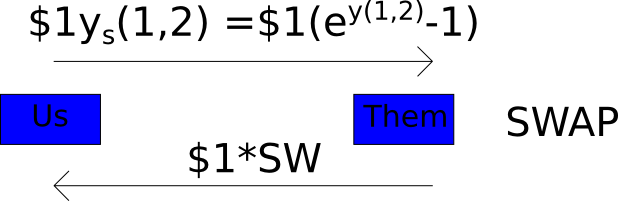
\includegraphics[width=3in]{pics/swap1P.png} \\
  \caption{Swap at t=2}
\label{swap1P}
\end{center}
\end{figure}

The answer comes from an arbitrage argument. We will hedge the floating payment with forwards and then find the swap rate that makes the combined value of all fixed and floating payments equal to zero. If they are not zero we have an arbitrage.

Say we recieve the fixed rate and pay the floating rate. The most obvious (and correct) hedge is a forward contract to borrow \$1 from $t=1$ to $t=2$. This rate is $f(1,2)$. At $t=1$ we lend out this \$1 for a year at the prevailing rate $y(1,2)$.

The table below gives the story of the swap and the hedge:

\begin{tiny}
\begin{tabular}{|c|c|c|}
\hline
time & contract/action & cashflow\\
\hline
0 & \begin{tabular}{c}Enter swap to pay $\$1*y_s(1,2)$ and receive $\$1*SW$\\ Enter forward to borrow \$1 at $f(1,2)$\\ \end{tabular} & 0\\
\hline
1 & \begin{tabular}{c}Borrow \$1 at $f(1,2)$\\ Lend \$1 at $y(1,2)$ \end{tabular} & 0\\
\hline
2 & & \begin{tabular}{c}Pay $\$1e^{f(1,2)}$ from loan\\ Receive $\$1e^{(y(1,2)}$ from loan\\ Pay $\$1y_s(1,2)$ from swap \\ Receive $\$1SW$ from swap\\  \end{tabular}\\
\hline
\end{tabular}
\end{tiny}

We can divide the cashflows into those coming from loans (including the loan at the forward rate) and the fixed and floating side of the swap. We'll also discount everything at $t=2$ by $y(0,2)$:

\begin{tiny}
\begin{tabular}{|c|c|c|c|}
\hline
time & value of loans & value of floating & value of fixed\\
\hline
0 & 0 & 0 & 0\\ 
1 & 0 & 0 & 0\\
2 & $e^{-y(0,2)}(\$1e^{y(1,2)}-\$1e^{f{1,2}})$ & $-e^{-y(0,2)}(\$1*y_s(1,2) = -e^{-y(0,2)}(\$1*(e^{y(1,2)}-1))$ & $e^{-y(0,2)}*\$1*SW$\\
\hline
\end{tabular}
\end{tiny}

Note that we substitute out $y_s$ with $y_s = e^y-1$. From here the swap rate $SW$ is easy to find. Since the portfolio is self financed it should give zero profit. The no-arbitrage condition is:

\begin{eqnarray*}
e^{-y(0,2)}(\$1e^{y(1,2)}-\$1e^{f{1,2}})-e^{-y(0,2)}(\$1*(e^{y(1,2)}-1))+e^{-y(0,2)}*\$1*SW = 0\\
\Rightarrow SW = e^{f(1,2)-1}
\end{eqnarray*}

The forward has done its job and offset the exposure to the floating rate. Figure \ref{swapAndHedge} tells the story:

\begin{figure}[htbp]
\begin{center}
  \includegraphics[width=3in]{pics/swapAndHedge.png} \\
  \caption{Swap and hedge combined at at $t=2$}
\label{swapAndHedge}
\end{center}
\end{figure}


\textbf{Example: Two period swap}\\

A two period swap adds one extra exchange: in period $t=3$ we exchange $\$1*y_s(2,3)$ for the swap rate $\$1*SW$ 

\begin{figure}[htbp]
\begin{center}
  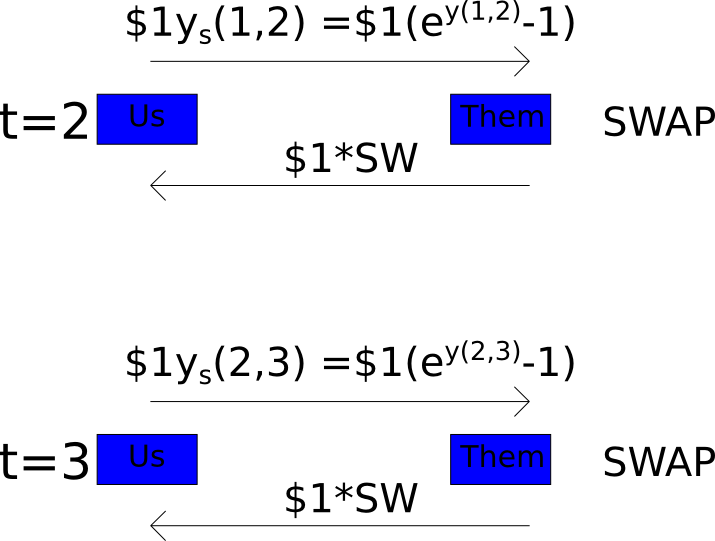
\includegraphics[width=3in]{pics/swap2P.png} \\
  \caption{Swap at $t=2$ and $t=3$}
\label{swap2P}
\end{center}
\end{figure}

Now we have to worry about two floating rates: $y_s(1,2)$ and $y_s(2,3)$. Since we pay the floating rate we need to borrow at the forward rate in $t=1$ and $t=2$ to offset. 

\begin{tiny}
\begin{tabular}{|c|c|c|}
\hline
time & contract/action & cashflow\\
\hline
0 & \begin{tabular}{c}Enter swap to pay $\$1*y_s(t-1,t)$ and receive $\$1*SW$ at $t=2,3$\\ Enter forwards to borrow \$1 at $f(t-1,t)$ for $t=2,3$\\ \end{tabular} & 0\\
\hline
1 & \begin{tabular}{c}Borrow \$1 at $f(1,2)$\\ Lend \$1 at $y(1,2)$ \end{tabular} & 0\\
\hline
2 &\begin{tabular}{c}\\ Borrow \$1 at $f(2,3)$\\ Lend \$1 at $y(2,3)$  \end{tabular}  & \begin{tabular}{c}Pay $\$1\exp(f(1,2))$ from loan\\ Receive $\$1\exp(y(1,2))$ from loan\\ Pay $\$1y_s(1,2)$ on swap \\ Receive $\$1SW$ from swap\\ \end{tabular}\\
\hline
3 & & \begin{tabular}{c}Pay $\$1\exp(f(2,3))$ from loan\\ Receive $\$1\exp(y(2,3))$ from loan\\ Pay $\$1y_s(2,3)$ on swap \\ Receive $\$1SW$ from swap\\ \end{tabular}\\
\hline
\end{tabular}\\
\end{tiny}

The discounted values of all the cashflows are summarised here 

\begin{tiny}
\begin{tabular}{|c|c|c|c|}
\hline
time & value of loans & value of floating & value of fixed\\
\hline
0 & 0 & 0 & 0\\ 
1 & 0 & 0 & 0\\
2 & $e^{-y(0,2)}(\$1e^{y(1,2)}-\$1e^{f(1,2)})$ & $-e^{-y(0,2)}\$1*y_s(1,2) = -e^{-y(0,2)}(\$1*(e^{y(1,2)}-1))$ & $e^{-y(0,2)}*\$1*SW$\\
3 & $e^{-y(0,3)}(\$1e^{y(2,3)}-\$1e^{f(2,3)})$ & $-e^{-y(0,3)}\$1*y_s(2,3) = -e^{-y(0,3)}(\$1*(e^{y(2,3)}-1))$ & $e^{-y(0,3)}*\$1*SW$\\
\hline
\end{tabular}
\end{tiny}

Since these are all in $t=0$ values we can sum up and set equal to zero to find the swap rate:

\[SW | \sum_{\tau=2}^3  e^{-y(0,\tau)}(1-e^{f(\tau-1,\tau)} +SW) = 0 \]

It's a simple matter to find $SW$ that satisfies this equation.

\subsection{The general formula}

The previous example easily generalises to an arbitrary number of periods. For a swap fixing at $t, t+1 \ldots T$ with anniversaries at $t+1,t+2,\ldots,T+1$ the swap price satisfies

\begin{eqnarray}
SW  | \sum_{\tau=t+1}^{T+1}  e^{-y(0,\tau)\tau}(e^{f(\tau-1,\tau)}-1 -SW) = 0  \label{swapprice}
\end{eqnarray}

Notice that since all cashflows are multiples of the notional value we can divide them out  without changing the result. 

This is an intuitive formula. It says \textbf{the sum of discounted differences between the (simple) forward rate and the swap rate should be zero}.

Some swaps pay fixed and floating rates at different times. It's easy to accommodate these. Let $N_F(t)$ and $N_L(t)$ be the fixed and floating notional values. Then 

\begin{eqnarray*}
SW  | \sum_{\tau=t+1}^{T+1}  e^{-y(0,\tau)\tau}N_L(t)(e^{f(\tau-1,\tau)}-1)  - e^{-y(0,\tau)\tau}N_F(t)SW = 0  \label{swapgeneral}
\end{eqnarray*}

We just have to remember to borrow $N_L(t)$ to construct the hedge. With swaps with asyncronous payments sometimes $N_L(t)$ and $N_F(t)$ will be zero. Our formula works fine with this.


\subsection{Worked example: 3 period swap}

\textit{Step 1: Calculate forward rates}\\

Suppose we have the following zero rates:\\
\begin{center}
\begin{tabular}{|c|c|}
  \hline
  % after \\: \hline or \cline{col1-col2} \cline{col3-col4} ...
  $t$ & $y(0,t)$ \\
  \hline
  1&0.05 \\
  2&0.06 \\
  3&0.09 \\
  4&0.08 \\
  5&0.07\\
  \hline
\end{tabular}
\end{center}
We can calculate the forward rates\\
\begin{center}
\begin{tabular}{|c|c|c|}
  \hline
  % after \\: \hline or \cline{col1-col2} \cline{col3-col4} ...
  $t$ & $y(0,t)$ & $f(t,t+1)$ \\
  \hline
  1&0.05 & 0.07\\
  2&0.06 & 0.15\\
  3&0.09 & 0.05 \\
  4&0.08 & 0.03\\
  \hline
\end{tabular}
\end{center}

\textit{Step 2: Construct discounted payoff and solve for swap rate}\\

We can use the general formula

\begin{eqnarray*}
\sum_{\tau=t+1}^{T+1}  e^{-y(0,\tau)}(e^{f(\tau-1,\tau)}-1 -SW) = 0 \\
\Rightarrow e^{-y(0,2)2}(e^{f(1,2)} - 1 - SW) + e^{-y(0,3)3}(e^{f(2,3)} - 1 - SW)+ e^{-y(0,4)4}(e^{f(3,4)} - 1 - SW) =0\\
\Rightarrow e^{-0.06*2}(e^{0.07} - 1 - SW) + e^{-0.09*3}(e^{0.015} - 1 - SW)+ e^{-0.08*4}(e^{0.05} - 1 - SW) =0\\
\Rightarrow SW = 0.094\\
\end{eqnarray*}

So the swap rate is 0.094.

\section{Questions}

\textbf{Question 1:}\\
Calculate the price for a bond that pays a coupon of \$10 per year for 5 years with a \$50 face value if the zero curve is constant at 3\%.

\textbf{Question 2:}\\
If the one year interest rate is $y(1) = 0.02$ and the 5 year interest rate is $y(5) = 0.03$ calculate the 4 year interest rate 1 year forward.

\textbf{Question 3:}\\
Suppose we have the following zero rates:\\
\begin{center}
\begin{tabular}{|c|c|}
  \hline
  % after \\: \hline or \cline{col1-col2} \cline{col3-col4} ...
  $t$ & $y(t)$ \\
  \hline
  1&0.05 \\
  2&0.06 \\
  3&0.07 \\
  4&0.08 \\
  5&0.09\\
  \hline
\end{tabular}
\end{center}


Consider a swap to receive \$1,000,000 times a some fixed swap rate $SW$ each year and pay \$1,000,000 times the one year zero rate $y(t-1,t)$ for four years starting at $t=2$. Calculate the no-arbitrage value of $SW$. (hint: you'll need to use a spreadsheet or mathematical package)



\section*{Appendix: Compounding}


So let's say I borrow \$1 and repay the loan in $t$ years from now with an annual rate of interest $ARI$ paid at the end of each year. I will repay

\[ \$1\underbrace{\left(1+\mbox{ARI}\right)\left(1+\mbox{ARI}\right)\ldots\left(1+\mbox{ARI}\right)}_{\mbox{t times}} \]


or

 \[\$1\left(1+\mbox{ARI}\right)^t \]

Suppose instead that the interest is paid semi-annually. I will now repay \[\$1\left(1+\frac{\mbox{ARI}}{2}\right)^{2t} \]

Suppose instead that the interest is paid quarterly. I will now repay \[\$1\left(1+\frac{\mbox{ARI}}{4}\right)^{4t} \]

Suppose I pay the interest every day. I will now repay \[\$1\left(1+\frac{\mbox{ARI}}{365}\right)^{365t} \]

As the frequency of repayment approaches infinity the repayments will approach \[\lim_{k\rightarrow\infty}\$1\left(1+\frac{\mbox{ARI}}{k}\right)^{kt} = \$1\exp(rt) \]

where $r$ is the \textit{continuously compounded interest rate}.

Say I borrow \$1 with $ARI = 1$ (100\% per year)

\begin{center}
\begin{tabular}{|p{8cm}|p{8cm}|}
  \hline
  % after \\: \hline or \cline{col1-col2} \cline{col3-col4} ...
  k (frequency of repayments) & repayments (one year)  \\
  \hline
  1 & $\$1\left(1+\frac{1}{1}\right)^{1*1} = \$2 $ \\
  4 & $\$1\left(1+\frac{1}{4}\right)^{4*1} = \$2.441406$ \\
  365 & $\$1\left(1+\frac{1}{365}\right)^{365*1} = \$2.714567$\\
  1000 & $\$1\left(1+\frac{1}{1000}\right)^{1000*1*} = \$2.716924 $  \\
  $\infty$ & $\lim_{k\rightarrow\infty}\$1\left(1+\frac{1}{k}\right)^{k*1} = \exp(1*1) \approx \$2.718282$\\
  \hline
\end{tabular}
\end{center}

The number 2.71828182845709... is called $e$. The expression $e^x$ is often written as $\exp(x)$. It is a very important number. If a variable $x$ grows at a rate $g$ for $t$ periods of compounded growth starting at $x(0)$ then its value at time $t$ will be

\[x(t) = x(0)\exp(gt) \]

Back to borrowing. Say I borrow \$1 with $ARI = 0.05$ (5\% per year) for one year
\begin{center}
\begin{tabular}{|p{8cm}|p{8cm}|}
  \hline
  % after \\: \hline or \cline{col1-col2} \cline{col3-col4} ...
  k (frequency of repayments) & repayments (one year) \\
  \hline
  1 & $\$1(1+\frac{0.05}{1})^{1*1} = \$1.05 $  \\
  4 & $\$1(1+\frac{0.05}{4})^{4*1} = \$1.050945$ \\
  365 & $\$1(1+\frac{0.05}{365})^{365*1} = \$1.0512675$ \\
  1000 & $\$1(1+\frac{0.05}{1000})^{1000*1} = \$1.051270 $ \\
  $\infty$ & $\lim_{k\rightarrow\infty}\$1(1+\frac{0.05}{k})^{k*1} = \exp(0.05*1) \approx \$1.051271$\\
  \hline
\end{tabular}
\end{center}

Say I borrow \$1 with $ARI = 0.05$ (5\% per year) for two years
\begin{center}
\begin{tabular}{|p{8cm}|p{8cm}|}
  \hline
  % after \\: \hline or \cline{col1-col2} \cline{col3-col4} ...
  k (frequency of repayments) & repayments (two years) \\
  \hline
  1 & $\$1(1+\frac{0.05}{1})^{1*2} = \$1.1025 $ \\
  4 & $\$1(1+\frac{0.05}{4})^{4*2} = \$1.104486$\\
  365 & $\$1(1+\frac{0.05}{365})^{365*2} = \$1.105163$ \\
  1000 &  $\$1(1+\frac{0.05}{1000})^{1000*2*} = \$1.105168 $  \\
  $\infty$ & $\lim_{k\rightarrow\infty}\$1(1+\frac{0.05}{k})^{k*2} = \exp(0.05*2) \approx \$1.105171$ \\
  \hline
\end{tabular}
\end{center}


We can convert between the $ARI$ and $y$ by comparing a discretely compounded loan with a continuously compounded loan
\begin{eqnarray*}
\mbox{discrete} & =\mbox{continuous}\\
\rightarrow \$1\left(1+\frac{\mbox{ARI}}{k}\right)^{kt} & = \exp(yt)
\end{eqnarray*}
\begin{equation}
\rightarrow y = k \ln \left(1+\frac{\mbox{ARI}}{k} \right)
\end{equation}


So in summary we have:

\textit{Discrete compounding:}

\[FV_{\mbox{discrete}} = \mbox{PV}\left(1+\frac{ARI}{k}\right)^{kt} \]

\textit{Continuous compounding:}

\[FV_{\mbox{continuous}} = \mbox{PV}\exp(yt) \]

We can also use this to discount payoffs which occur in the future by:

\[FV\exp(-yt) = \mbox{PV} \]


\textit{Converting between discrete and continuous compounding:}

\[FV_{\mbox{continuous}} = FV_{\mbox{discrete}} \rightarrow y = k \ln \left(1+\frac{ARI}{k} \right)\]

where
\begin{itemize}
\item PV: present value of loan\\
\item FV: future value of loan\\
\item ARI: annual rate of interest (discrete)\\
\item $k$: number of compounding periods per year\\
\item $t$: number of years\\
\item $y$: continuously compounded interest rate
\end{itemize}





